\section{Discussion}
The performance evaluation of \papertitle\hspace{2pt} shows a satisfying result with usage data collected from a variety of participants.
Because our implementation is based on RDF, it is very easy to adapt to new user behavior with a small amount of training data.
In this section, we discuss user behavior, limitations and possible improvements of this prototype.

\subsection{Observation of User Behavior}
All of the participants used only one finger to move cursors without any instructions.
Participants reported that they directly adapted their previous experience of using a traditional touchpad, so they used only one finger to touch on the surface of \papertitle.
While we expected most of the users would rest their fingers on the surface of the keyboard, we observed that a large part (19 out of 30) of the users lifted their left hand while using touchpad function(see Figure~\ref{fig:pedal}.B).
None of the participants could explain the cause of this behavior. Our explanation is that users may treat the whole keyboard as a long touchpad so they remove all the obstacles before using it.
Although one-third of the participants did not lift their non-dominant hands while using trackpad, the overall correctness of our classifier remain high (98\%), so it is believed that the classifier can distinguish touch from typing whether users rest their non-dominant hands on the keyboard or not.
In the meanwhile, most of the users tried to use the touchpad in a very small area, about 3x3 cm for shorter movement. 
20 of 30 users operated the cursor on the center area of the keyboard, 9 users operated on the center of the right side, the other 1 user operated on the bottom of right side.
% \begin{figure}[!ht]
% \centering
% 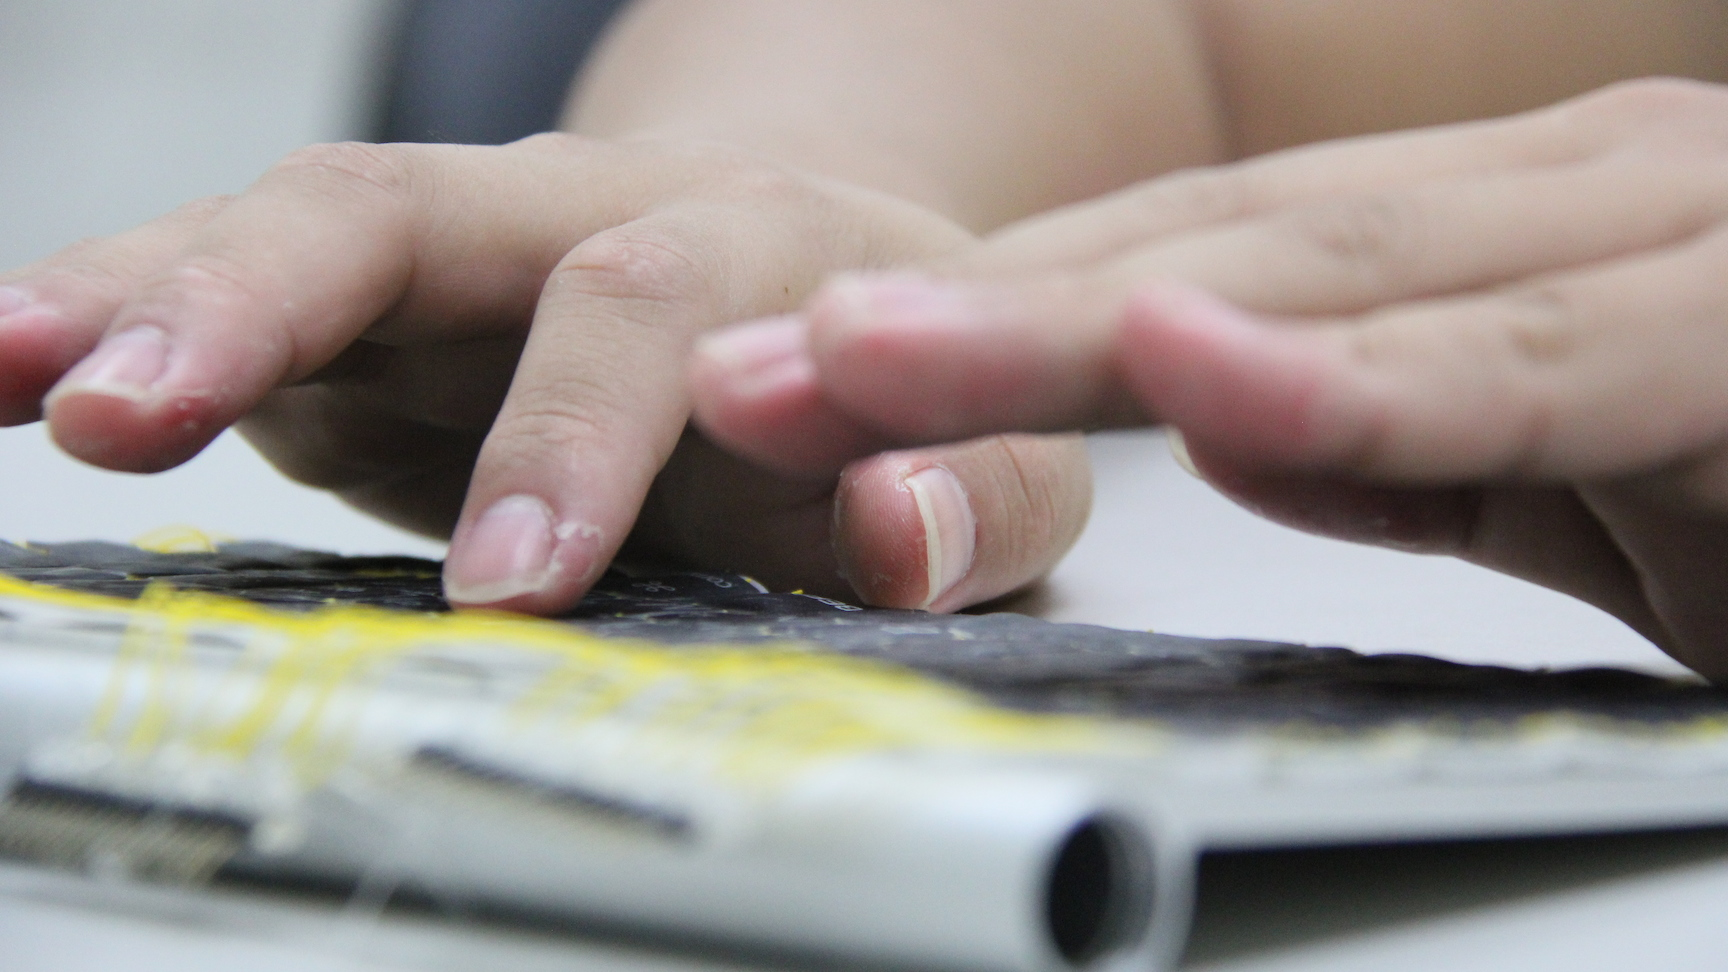
\includegraphics[width=0.8\columnwidth]{figures/figure4.jpg}
% \caption{A majority of participants raised their left hand and use one finger of right hand to perform cursor movement in the trackpad mode.}
% \label{fig:figure4}
% \end{figure}


\subsection{Uneven Touch Surface}
Many users reported that the surface of \papertitle\hspace{2pt} is too uneven to perform smooth cursor pointing operations.
The user's fingers may get stuck between the key caps, which make it harder to move his finger to the desired position.
This drawback can be solved with some physical modification, such as adding a mechanical structure to lift the case of a Chiclet keyboard to the top of key caps, forming a flat and smooth platform for users to perform a surface operation. 
% We further built an automatically lift keyboard with our automatic mode switching predictor. We will conduct an usability testing with this form factor in the future.

\subsection{Higher Frame Rate and Resolution}
The frame rate of the current prototype may be too low for some time-critical interactions.
There are two major bottlenecks of current implementations: sampling speed of the lock-in amplifier and the speed of MCU.
Currently, sampling speed of the lock-in amplifier is bounded by two factors: the RC time constant of RC low-pass filter and sampling speed of ADC.
Both of them can be improved by using better implementation options, which require modification of the hardware design.
On the other hand, we can save more MCU computing power by dividing the raster scanning process into two stages.
We can scan a lower resolution image first, calculate possible touch blobs position with it, and perform a higher resolution raster scanning around touched blobs.
This modified process is faster in most of the cases (the number of touched blobs $<$ 5), and does not sacrifice precision.
As a result, the frame rate can be higher without modifying the hardware setup.
%Final: reviewer 問gesture
% move to conclusion
%\subsection{Future Work}
%Now, our system can automatically switch between trackpad mode and typing mode with very high accuracy. However, we only enable pointing and 2-finger scrolling gesture in trackpad mode. In the future, we are planning to implement gesture recognizing system to recognize more multi-touch gestures, such as, swipe, and pinch on our system.